\documentclass{report}

\usepackage[left=2.5cm,right=2.5cm,top=3cm,bottom=3cm]{geometry}
\usepackage{amsmath}
\usepackage{amssymb}
\usepackage{xcolor}
\usepackage{graphicx}
\usepackage{algorithm}
\usepackage{algpseudocode}
\usepackage{url}
\usepackage[hidelinks,colorlinks]{hyperref}
\usepackage[italian]{babel}
\selectlanguage{\italian}
\usepackage{subcaption}


% Space for float placement
\def\topfraction{1}
\def\bottomfraction{.5}
\def\textfraction{0}
\def\floatpagefraction{1}

% Pagestyle
\pagestyle{myheadings}
\renewcommand{\chaptermark}[1]{\markboth{#1}{} }
\renewcommand{\sectionmark}[1]{\markright{#1}{} }

\usepackage{listings}
\definecolor{backcolour}{rgb}{0.95,0.95,0.92}
\definecolor{codecolor}{rgb}{0.2,0.2,0.7}
\definecolor{keywordcolor}{rgb}{1,0,0}
\definecolor{numbercolor}{rgb}{0.5,0.5,0.5}
\definecolor{lnkcolor}{rgb}{0.1,0.1,1.0}
\definecolor{lnkcolor2}{rgb}{0,0,0}

\lstdefinestyle{mystyle}{
    backgroundcolor=\color{backcolour},   
    commentstyle=\color{codecolor},
    keywordstyle=\color{keywordcolor},
    numberstyle=\tiny\color{numbercolor},
    stringstyle=\color{codecolor},
    basicstyle=\ttfamily\small\color{codecolor},
    breakatwhitespace=false,         
    breaklines=true,                 
    captionpos=b,                    
    keepspaces=true,                 
    numbers=left,                    
    numbersep=5pt,                  
    showspaces=false,                
    showstringspaces=false,
    showtabs=false,                  
    tabsize=2
}

\lstset{style=mystyle}

\hypersetup{
linkcolor=lnkcolor2
,citecolor=lnkcolor
,filecolor=lnkcolor
,urlcolor=lnkcolor
,menucolor=lnkcolor
,runcolor=lnkcolor
%,linkbordercolor=
%,citebordercolor=
%,filebordercolor=
%,urlbordercolor=
%,menubordercolor=
%,runbordercolor=
}

\setlength{\parskip}{1ex}
\setlength{\parindent}{0pt}

%\renewcommand{\familydefault}{\sfdefault}

\newcommand{\textttt}[1]{{\color{codecolor}\texttt{#1}}}

\begin{document}

\thispagestyle{empty}
\begin{center}
    \Large Corso di Laurea in Ingegneria Gestionale\\
\Large Classe L-8\\[2cm]


\includegraphics[width=12cm]{images/Logo_PoliTo_scritta.png}

\vspace*{2cm}

{\Huge \bfseries Applicazione per la creazione di un itinerario gastronomico personalizzato}

\vfill

{\Large \bfseries Relatore\hfill Candidato}\\
{\Large Fulvio Corno \hfill Lorenzo Grivet Talocia}

\vspace*{1cm}
{\Large Ottobre 2024}

\end{center}


\tableofcontents

\hypersetup{
linkcolor=lnkcolor
}

\chapter{Proposta di progetto}\label{cap_proposta}

\section{Titolo della proposta}\label{sec_titolo}
Applicazione per la creazione di un itinerario gastronomico personalizzato

\section{Descrizione del problema proposto}\label{sec_descrizione}
Lo scopo dell'applicazione è quello di generare automaticamente un percorso gastronomico personalizzato all'interno di una città desiderata, elaborato rispettando i vincoli scelti dall'utente, in modo tale da massimizzare l'indicatore di qualità dei ristoranti. L'utente può infatti, per ogni città scelta, selezionare le proprie preferenze di tipologia di cucina, prezzo e le proprie eventuali intolleranze alimentari. 

Il programma offre inoltre altre funzionalità come la ricerca dei migliori ristoranti che rispettano i vincoli inseriti che l'utente può inserire all'interno del proprio percorso.

\section{Descrizione della rilevanza gestionale del problema}\label{sec_rilevanza}
Il programma che si vuole implementare si sviluppa intorno alla creazione di una sequenza di ristoranti che sia la migliore possibile per l'utente che lo utilizza. Il servizio quindi fornito dall'applicazione, che utilizza come sorgente dati un estratto delle informazioni presenti sulla nota piattaforma di viaggi TripAdvisor, aggiunge una funzionalità che ora il sito non offre.  

\section{Descrizione del data-set per la valutazione}
Il dataset utilizzato è stato ottenuto raccogliendo le informazioni sui locali presenti sulla piattaforma di viaggi TripAdvisor. I dati riguardano più di 125000 ristoranti oltre ad informazioni sulla città, tipo di cucina, rating, recensioni e fascia di prezzo.

Il dataset è disponibile all'indirizzo: \url{www.kaggle.com/datasets/damienbeneschi/krakow-ta-restaurans-data-raw}.
Sono state apportate alcune piccole modifiche rispetto alla fonte originale.

\section{Descrizione preliminare degli algoritmi coinvolti}\label{sec_algoritmi}
Il software è realizzato in linguaggio Python sfruttando il pacchetto Flet per l'interfaccia grafica.
La prima parte dell'applicazione sfrutta interrogazioni del database mediante query SQL mentre la seconda utilizza algoritmi più complessi. Il programma costruisce un grafo, servendosi del pacchetto Python NetworkX, e si serve di un algoritmo ricorsivo per calcolare l'itinerario.

\section{Descrizione preliminare delle funzionalità previste per l’applicazione software}\label{sec_funzionalità}
All'apertura del programma l'interfaccia grafica presenta due schede. 
La prima permette, impostando dei filtri, di effettuare delle interrogazioni del database ricavando i migliori dieci ristoranti che rispettino i vincoli inseriti. 
E' successivamente possibile aggiungere uno o più ristoranti appena trovati alla propria lista personale, la quale può essere opportunamente modificata in qualunque momento.

La seconda parte si occupa invece, sfruttando un algoritmo ricorsivo, di costruire un itinerario tra i ristoranti (di lunghezza impostata dall'utente) in modo tale da scegliere i migliori possibili. E' inoltre possibile specificare eventuali intolleranze alimentari e scegliere alcune tra le tante disponibili tipologie di cucina. L'applicazione si assicurerà di calcolare il percorso in modo da evitare due ristoranti consecutivi che presentino le stesse tipologie di cucina.


\chapter{Descrizione del problema affrontato}\label{cap_problema}

\section{Contesto}\label{sec_contesto}
L'applicazione realizzata propone un utile strumento che può essere di aiuto agli utenti semplificando e filtrando le ricerche e la navigazione tra il vasto numero di informazioni disponibili sulla rete. 

Il meccanismo delle recensioni online, in particolare, è diventato uno strumento essenziale per la valutazione di un ristorante da parte del pubblico, andando a costituire la colonna portante di tante piattaforme come TripAdvisor, fonte del data-set su cui si basa l'applicazione.
Tuttavia, il grande numero di recensioni e di informazioni disponibili rischia di generare un effetto controproducente, ovvero confondere gli utenti senza riuscire ad far risaltare le indicazioni importanti.

Questa è la criticità che la prima parte dell'applicazione si propone di risolvere, rendendo disponibile uno strumento che consenta all'utente di selezionare le proprie preferenze, o di non selezionarne nessuna, scartando un'enorme gamma di informazioni che non vengono presentate.

La seconda parte dell'applicazione risolve, invece, la difficoltà di pianificare autonomamente un itinerario di ristoranti in cui recarsi semplicemente esprimendo le proprie preferenze. 

\section{Input e output}
Durante la propria esecuzione, l'applicazione riceve in input due tipologie di indicazioni Il data-set contenente tutte le informazioni dei ristoranti di trentuno città europee e, da parte dell'utente, il programma recepisce una grande serie di informazioni: preferenze di tipologia di cucina, la durata del soggiorno nella città scelta, la fascia di prezzo cercata ed eventualmente le intolleranze o abitudini alimentari dei clienti (diete vegetariane, celiache o halal).

L'output che è restituito si concentra sempre sul ricavare la miglior soluzione rispettando i vincoli inseriti, così nel caso della ricerca dei migliori ristoranti come nella ricerca dell'Itinerario gastronomico.

\section{Potenzialità e criticità}
Le potenzialità dell'applicazione si concentrano sulla semplificazione ed efficienza della navigazione dell'utente.
Le criticità possono, invece, essere legate alla veridicità delle informazioni derivate dalle recensioni che, per loro natura, non garantiscono di essere sicuramente affidabili.


\chapter{Descrizione del dataset}\label{cap_dataset}
Il data-set utilizzato si compone di una tabella "ta\_restaurants\_curated" contenente informazioni riguardo ai ristoranti registrati su TripAdvisor di trentuno città europee, in totale sono presenti più di 120 mila ristoranti in tutta Europa. Il data-set è stato scaricato all'indirizzo: \url{https://www.kaggle.com/datasets/damienbeneschi/krakow-ta-restaurans-data-raw}
La tabella "ta\_restaurants\_curated" contiene, per ogni ristorante:
\begin{itemize}
    \item \textbf{Nome del ristorante}: Il nome del ristorante.
    \item \textbf{Città}: La città in cui si trova il ristorante.
    \item \textbf{Tipologie di cucina}: Un elenco di tipologie di cucina offerte dal ristorante.
    \item \textbf{Ranking}: La posizione del ristorante nella classifica della propria città.
    \item \textbf{Rating}: Un numero tra 1 e 5 che rappresenta il valore medio delle recensioni date dagli utenti.
    \item \textbf{Range di prezzo}: Suddiviso in tre classi che misurano in modo approssimato quanto è caro il ristorante.
    \item \textbf{Numero di recensioni degli utenti}: Il numero totale di recensioni degli utenti.
    \item \textbf{Esempio di due recensioni}: Due recensioni prese come esempio.
    \item \textbf{URL TripAdvisor}: Il link URL collegato alla pagina di TripAdvisor.com.
    \item \textbf{ID univoco}: Un ID univoco per ogni ristorante.
\end{itemize}


\chapter{Descrizione algoritmi utilizzati}\label{cap_algoritmi}

\section{Pattern MVC e DAO}\label{sec_MVC}
Il software è stato realizzato in Python seguendo il pattern MVC (\textit{Model, View, Controller}): 
\begin{itemize}
    \item \textit{View}: la view si occupa della rappresentazione grafica delle informazioni ricevute dal controller.
    \item \textit{Controller}: il controller gestisce l'interazione tra gli input dell'utente ottenuti tramite la view e la logica del programma interrogando il model.
    \item \textit{Model}: il model gestisce la logica applicativa del programma, l'accesso ai dati e l'elaborazione 
\end{itemize}
Questo garantisce la separazione delle funzionalità di ciascuna classe aumentando la scalabilità del codice.

L'interazione con il database è invece affidata al pattern DAO (\textit{Data Access Object}) che è utilizzato per fornire un'interfaccia unificata per l'accesso ai dati, in modo che l'applicazione non debba preoccuparsi dell'estrazione dei dati

\section{Algoritmi principali utilizzati}\label{sec_algoritmi}

\subsection{Compilazione automatica dei parametri}\label{sec2_parametri}
All'avvio dell'applicazione l'utente è tenuto ad effettuare tramite dei menu a tendina le prime due scelte: una città (all'interno delle trentuno che sono presenti nel data-set) e una fascia di prezzo (è anche possibile scegliere di non specificare una fascia di prezzo in particolare). Una volta selezionate le scelte, si compileranno automaticamente i campi di testo facenti riferimento al minimo e massimo Rating disponibile per la combinazione di città e fascia di prezzo scelta. Questi due valori sono estratti dal database tramite la seguente query SQL parametrica:
\begin{lstlisting}[language=SQL, caption={Query SQL per estrarre il minimo e massimo Rating}]
select min(t.Rating),max(t.Rating)
from ta_restaurants_curated t
where t.City =%s
and t.Price_Range = %s
and t.Rating >0
and not isnull(t.Number_of_Reviews)    
\end{lstlisting}
All'utente è comunque lasciata la possibilità di compilare i campi manualmente e il programma, nel caso sia inserito un input non consentito, creerà un messaggio di errore.

Ugualmente, il menu a tendina che permette di selezionare una tipologia di cucina (oppure di sceglierne qualsiasi) sarà automaticamente popolato nel momento in cui l'utente modifica i parametri precedentemente citati; anche una modifica del Rating può comportare l'eliminazione o l'aggiunta di una o più tipologie di cucina che è possibile selezionare. La query SQL sfruttata è la seguente:
\begin{lstlisting}[language=SQL, caption={Query SQL per estrarre le tipologie di cucina}]
select Cuisine_Style 
from ta_restaurants_curated t
where City =%s
and Price_Range = %s
and Rating >=%s
and Rating <=%s
and not isnull(t.Number_of_Reviews)
and not (Cuisine_Style like "%Vegan Options%" or Cuisine_Style like "%Vegetarian Friendly%" or Cuisine_Style like "%Gluten Free Options%")
\end{lstlisting}

\subsection{Salvataggio delle scelte}\label{sec2_eventi}
Ogni volta che l'utente effettua una scelta da un menu a tendina o digita del testo negli appositi campi, l'applicazione, grazie al \textit{Controller}, memorizza gli input in variabili di classe che sono utilizzate per interagire con il \textit{Model}. Il codice Python è simile per ognuno dei parametri di input:
\begin{lstlisting}[language=Python,caption=Codice per memorizzare input dell'utente]
def getSelectedPrezzo(self,e):
    if e.control.data is None:
        pass
    else:
        self.selectedPrezzo=e.control.data

        self.view.ddPrezzo_R.value=self.selectedPrezzo

        if self.selectedCitta is not None:
            self.fillRating(self.selectedCitta, self.selectedPrezzo)
\end{lstlisting}
La funzione \textit{getSelectedPrezzo} viene chiamata dal codice quando l'utente seleziona dal menu una fascia di prezzo, andando così a modificare la variabile \textit{selectedPrezzo} del \textit{Controller}. Le ultime due righe, inoltre, verificano che se l'utente abbia già selezionato la città e, nel caso sia già stata scelta, esegue la funzione \textit{fillRating} che, come precedentemente spiegato, compila automaticamente i campi relativi ai minimo e massimo \textit{Rating}.

\subsection{Ricerca dei migliori ristoranti}\label{sec2_migliori}
Una volta effettuate le scelte, l'utente può premere sul bottone \textit{Trova Migliori} comandando all'applicazione di stampare a video i migliori dieci ristoranti che rispettano i vincoli inseriti. Anche quest'ultima ricerca è stata eseguita tramite una query SQL, il codice del \textit{Model} risulta quindi molto semplice e rapido:
\begin{lstlisting}[language=Python,caption=Codice per ricavare migliori dieci ristoranti]
def getTopDieci(self,citta,prezzo,min,max,cucina):
    res=DAO.getTopDieciDAO(citta,prezzo,min,max,cucina)
    return res
\end{lstlisting}


\subsection{Creazione del grafo}\label{sec2_grafo}
Alla pressione del bottone \textit{Calcola}, una volta che le scelte sono già state effettuate, l'applicazione effettua una query per estrarre dal database i ristoranti filtrati secondo i vincoli inseriti dall'utente, eliminando quelli che hanno un fattore, dato dal prodotto di \textit{Rating} e numero di recensioni, inferiore alla media. Grazie a questa cernita il numero di operazioni che il programma deve svolgere si riduce notevolmente elminando i ristoranti che, in ogni caso, non sarebbero rientrati nell'itinerario migliore.

Una volta trovati gli effettivi nodi del grafo, il programma corregge il \textit{Rating} di ciascuno di questi tenendo in considerazione del numero di recensioni ricevute: la correzione è effettuata tramite il calcolo di un valore da sommare al \textit{Rating}. Inzialmente ogni ristorante è assegnato all'interno di una classe in base al numero di recensioni ottenute:
\begin{lstlisting}[language=Python,caption=funzione che assegna classe ad un ristorante in base al numero di recensioni]
def assegnaClasse(self, r):
    if r.Number_of_Reviews < 5:
        r.classe=0
    elif r.Number_of_Reviews >=5 and r.Number_of_Reviews<30:
        r.classe=1
    elif r.Number_of_Reviews>=30 and r.Number_of_Reviews<100:
        r.classe=2
    elif r.Number_of_Reviews>=100 and r.Number_of_Reviews<500:
        r.classe=3
    elif r.Number_of_Reviews>=500:
        r.classe=4
\end{lstlisting}
Successivamente è calcolato il termine additivo e modificato il \textit{Rating} del ristorante (r):
\begin{align}
\text{deltaRating} = r.\text{Rating} - 3\\
\text{correzione} = \text{deltaRating} \times r.\text{classe} \times 0.1\\
r.\text{Rating} = r.\text{Rating} + \text{correzione}
\end{align}

La creazione del grafo è uno dei passaggi più delicati siccome da questa dipende la parte centrale dell'applicazione, ovvero la ricerca dell'itinerario. La funzione \textit{creaGrafo} è responsabile, servendosi della libreria \textit{NetworkX}, della creazione del grafo. Inizialmente viene creato il grafo (non orientato e non pesato) e, successivamente, sono aggiunti i nodi precedentemente ricavati tramite il metodo di \textit{NetworkX} \textit{add\_nodes\_from}.

Dal momento che l'itinerario cercato non può avere due ristoranti considerati simili in due giorni consecutivi, due nodi sono collegati da un arco se almeno uno dei due ristoranti ha più di metà delle sue tipologie di cucina diverse dall'altro. In questo modo è possibile riconoscere due ristoranti come differenti nonostante presentino un numero limitato di tipologie di cucina in comune.

%due ottenere una sequenza di locali differenti anche se poche tipologie di cucina coincidono.
%DA CAMBIARE*********************************************%

Infine, con l'ultima riga del codice sottostante, gli archi sono aggiunti al grafo tramite il metodo di \textit{NetworkX} \textit{add\_edges\_from}.
\begin{lstlisting}[language=Python,caption=Funzione che crea il grafo]
def creaGrafo(self,nodi):
    self.grafo=nx.Graph()
    self.grafo.add_nodes_from(nodi)
    archi=[]
    for i in range(len(nodi)):
        for j in range(i+1,len(nodi)):
            a=nodi[i]
            b=nodi[j]

            d=len(a.setCucine-b.setCucine)
            e=len(b.setCucine-a.setCucine)

            if d>math.ceil(len(a.setCucine)/2) or e>math.ceil(len(b.setCucine)/2): 
                daAggiungere=True
            else:
                daAggiungere=False

            if daAggiungere:
                archi.append((a,b))

    self.grafo.add_edges_from(archi)
\end{lstlisting}



\subsection{Algoritmo di ricorsione}\label{sec2_ricorsione}
L'algoritmo ricorsivo utilizzato dall'applicazione per la creazione dell'itinerario è il più complesso tra quelli descritti; nonostante averne già scartati una parte, come precentemente descritto, il numero di ristoranti eleggibili nel percorso può essere molto alto quindi, inevitabilmente, il tempo di calcolo del programma può subire grossi aumenti.
\label{codice_ricorsione}
\begin{lstlisting}[language=Python,caption=Ricorsione per ricavare migliore itinerario]
def ricorsione(self, parziale, ultimo,giorni):
  
    ammissibili = self.getAmmissibili(parziale,ultimo,giorni)

    if self.isTerminale(parziale,ammissibili):
        c=self.calcolaPuntaggio(parziale)

        if c> self.maxPunteggio:
            print(c)
            self.solBest=copy.deepcopy(parziale)
            self.maxPunteggio=c
            return
    else:
        for a in ammissibili:
            parziale.append(a)
            self.ricorsione(parziale,a,giorni)
            parziale.pop()
\end{lstlisting}

Inizialmente sono trovati i nodi ammissibili tramite la funzione \textit{getAmmissibili} che restituisce i successori del nodo di partenza che non siano già presenti nella soluzione parziale e che abbiano un \textit{Rating} minore, in modo da ottenere il miglior ristorante all'inizio del percorso:
\begin{lstlisting}[language=Python,caption=Funzione che restituisce i nodi ammissibili nella soluzione parziale]
def getAmmissibili(self, parziale, ultimo,giorni):
    amm=[]
    if len(parziale)==giorni:
        return amm
    else:
        vic= list(self.grafo.neighbors(ultimo))
        for a in vic:
            if a not in parziale:
                if ultimo.Ranking < a.Ranking:
                    amm.append(a)
        return amm
\end{lstlisting}

Successivamente se la soluzione parziale trovata è terminale, ovvero non ci sono nodi ammissibili, viene calcolato il punteggio, dato dalla somma dei \textit{Rating}:
\begin{lstlisting}[language=Python,caption=Funzione per il calcolo del punteggio]
def calcolaPuntaggio(self, parziale):
    somma=0
    for i in parziale:
        somma+=i.Rating
    return somma
\end{lstlisting}
Se il punteggio è maggiore del massimo precedentemente trovato, la soluzione è memorizzata come la migliore.

Se la soluzione non è terminale, il programma continua ad aggiungere ristoranti alla lista tra gli ammissibili, eseguendo una ricorsione ad ogni aggiunta di un nodo fino al raggiungimento del numero massimo di ristoranti concesso, pari al numero di giorni che l'utente imposta.

Il comando \textit{parziale.pop} presente all'ultima riga della ricorsione (\ref{codice_ricorsione}) garantisce il \textit{backtracking} dell'algoritmo per poter esplorare sistematicamente tutte le possibilità di soluzione.


\chapter{Diagramma delle classi}\label{cap_diagramma}
Il \textit{Model} e il \textit{Controller} sono le classi principali.
\begin{figure}[h!]
    \centering
    \resizebox{0.8\textwidth}{!}{ 
        \begin{minipage}{\textwidth}
            \begin{subfigure}[h]{0.45\textwidth}
                \centering
                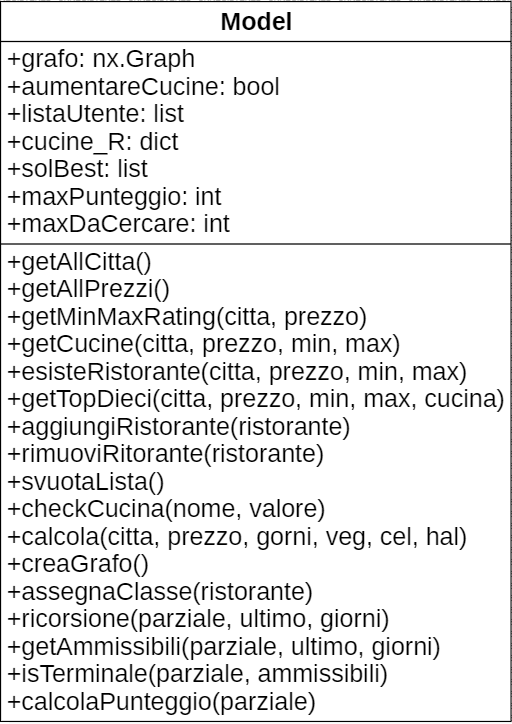
\includegraphics[width=\textwidth]{images/model.png}
                \caption{Model}
                \label{fig:model}
            \end{subfigure}
            \hfill
            \begin{subfigure}[h]{0.45\textwidth}
                \centering
                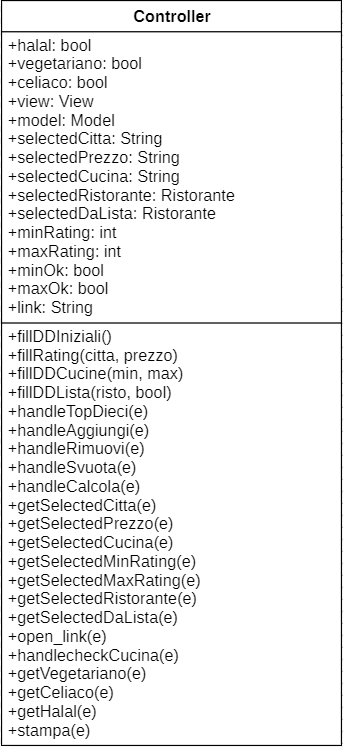
\includegraphics[width=\textwidth]{images/controller.png}
                \caption{Controller}
                \label{fig:controller}
            \end{subfigure}
        \end{minipage}
    }
    \caption{Diagramma delle classi}
    \label{fig:diagramma}
\end{figure}


\chapter{Videate dell'applicazione}\label{cap_videate}
\begin{figure}[h]
    \centering
    \fbox{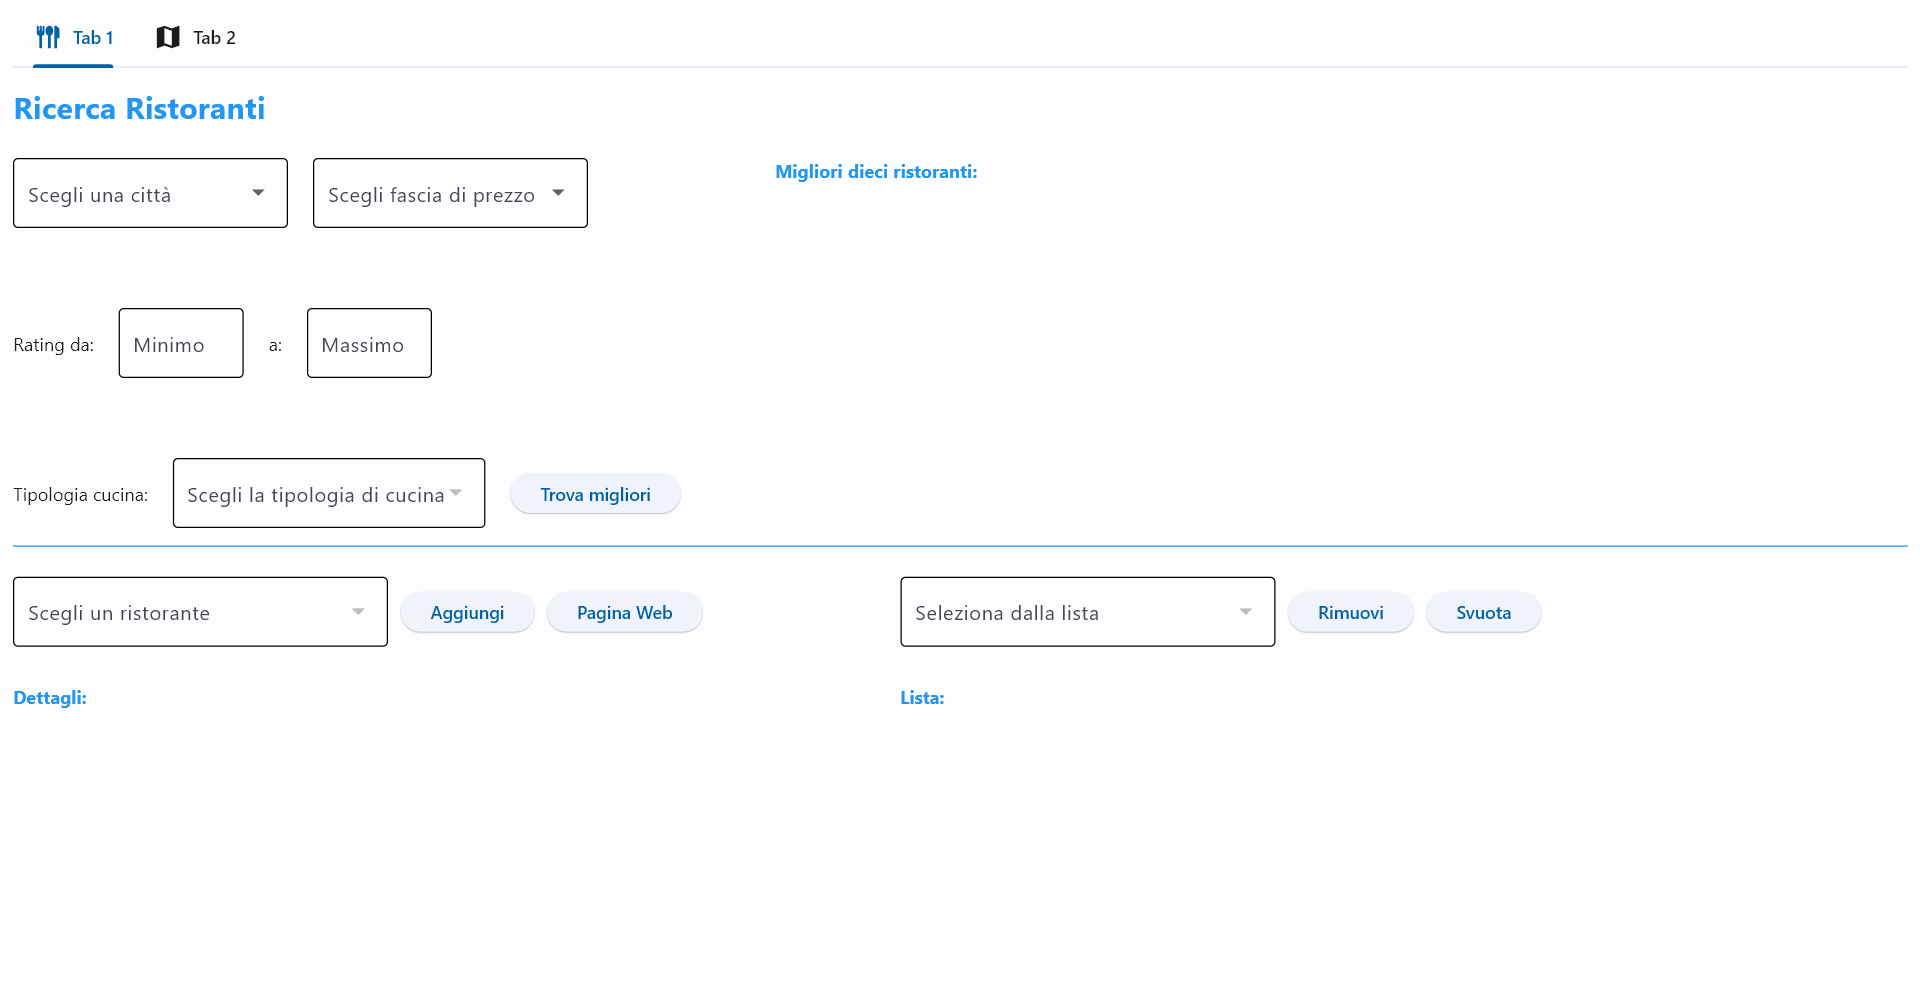
\includegraphics[width=1\textwidth]{images/screen_tesi1.png}}
    \caption{Prima schermata all'avvio dell'applicazione}
    \label{fig_schermata1}
\end{figure}

\begin{figure}[h]
    \centering
    \fbox{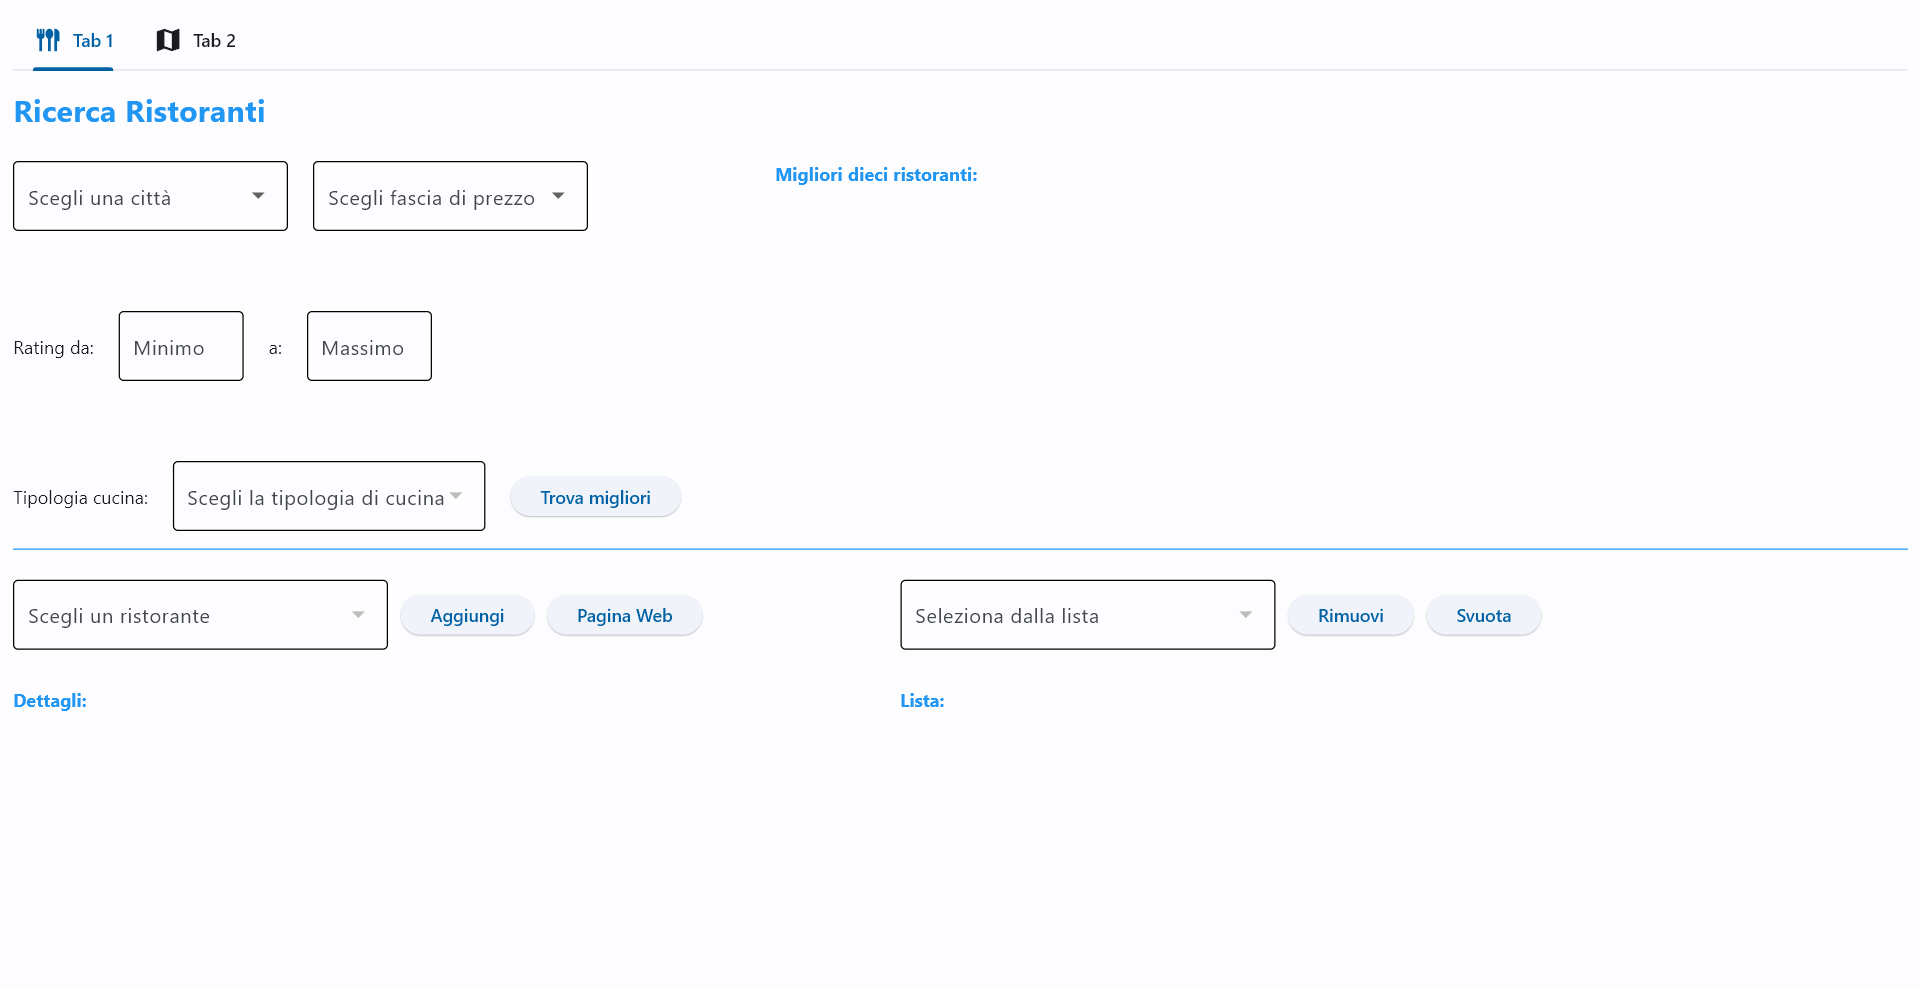
\includegraphics[width=1\textwidth]{images/screen_tesi2.png}}
    \caption{Seconda schermata all'avvio dell'applicazione}
    \label{fig_schermata1}
\end{figure}

\begin{figure}[h]
    \centering
    \fbox{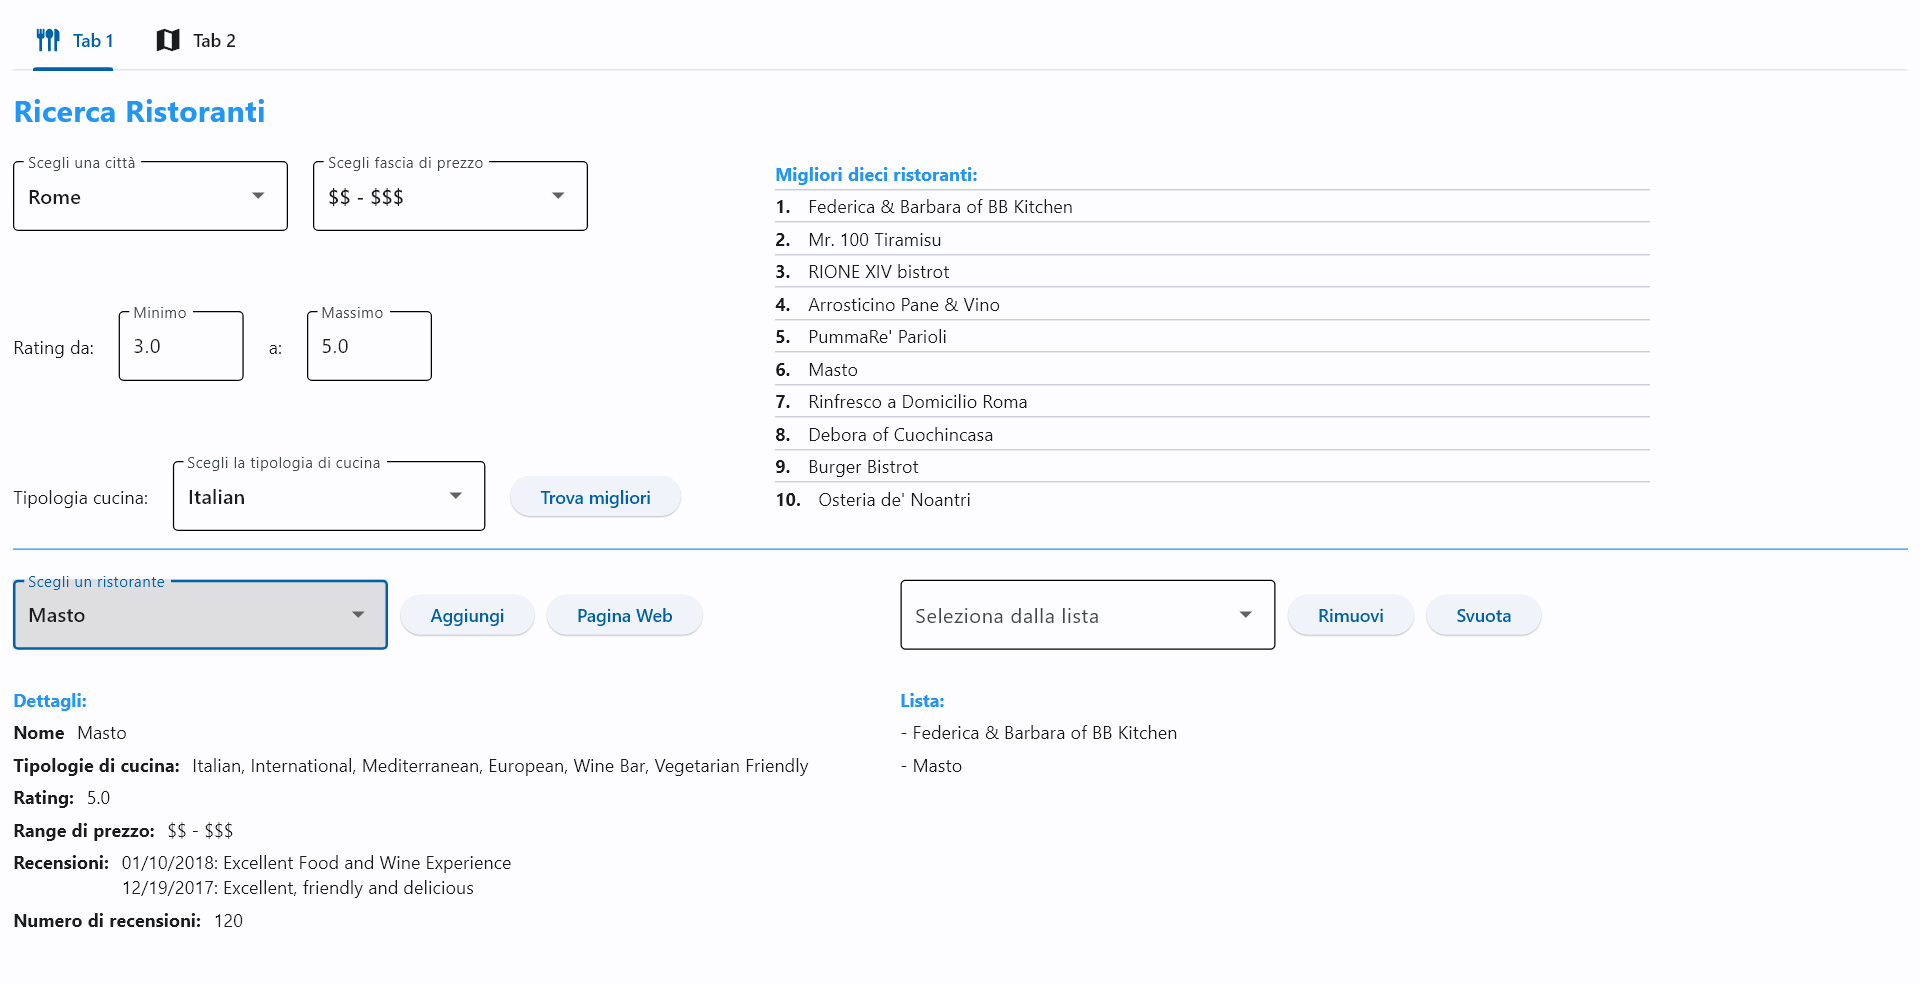
\includegraphics[width=1\textwidth]{images/screen_tesi7.png}}
    \caption{Prima schermata dopo utilizzo dell'utente}
    \label{fig_schermata1}
\end{figure}

\begin{figure}[h]
    \centering
    \fbox{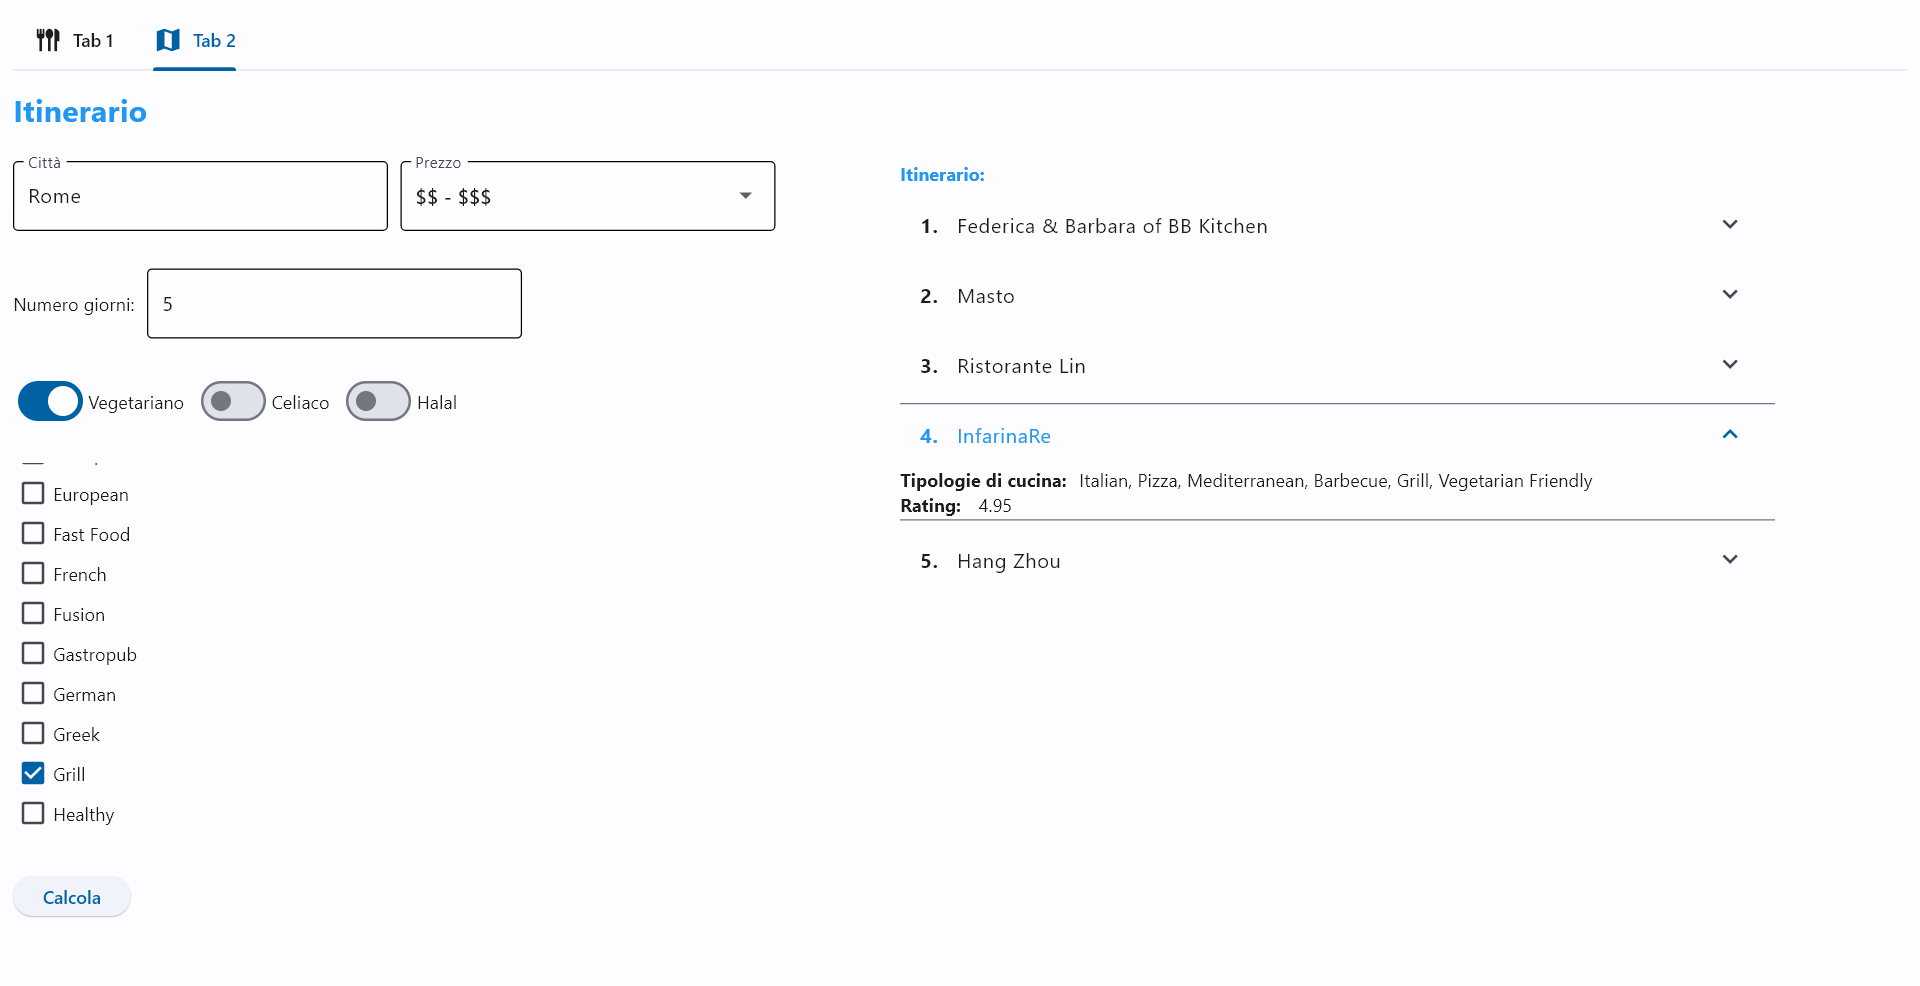
\includegraphics[width=1\textwidth]{images/screen_tesi6.png}}
    \caption{Seconda schermata dopo utilizzo dell'utente}
    \label{fig_schermata1}
\end{figure}



\chapter{Risultati sperimentali}\label{cap_risultati}

\section{Utilizzo di SQL}
L'utilizzo di SQL è molto vantaggioso: è infatti evidente come si riduca, quasi dimezzandosi, il tempo impegato dallo svolgimento della query rispetto al corrispondente codice in Python utile per raggiungere lo stesso obiettivo. Il grafico sottostante rappresenta la relazione tra tutte le possibili combinazioni di città e fascia di prezzo e il tempo impiegato rispettivamente da SQL (in viola) e da Python (in verde) per ricavare il risultato.
\begin{figure}[h]
    \centering
    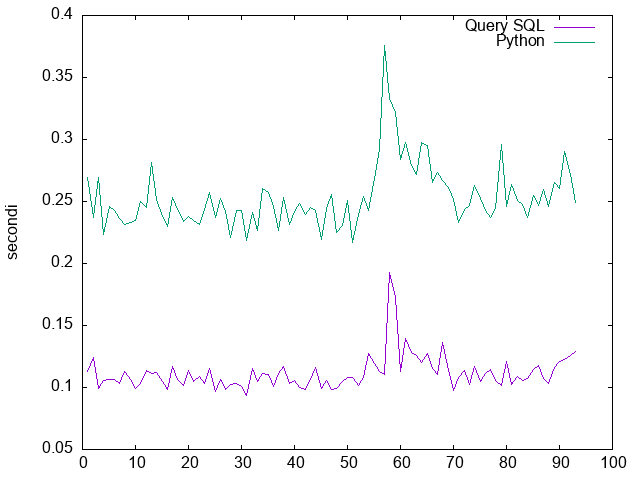
\includegraphics[width=0.8\textwidth]{images/graficoTempiTesi.png}
    \caption{Grafico tempi SQL-Python}
\end{figure}

\section{Algoritmo ricorsivo}
La ricorsione è, a livello di complessità computazionale, sicuramente l'algoritmo che ha un impatto maggiore sull'esecuzione del programma. Se il numero di dati cresce, di conseguenza si verificherà un sensibile aumento dei tempi impiegati dall'algoritmo ricorsivo. Il grafico seguente evidenzia il tempo (in secondi) impiegato dall'applicazione per l'esecuzione del codice, per ognuna delle tre fasce di prezzo. Il test è stato effettuato richiedendo un itinerario di cinque giorni, scegliendo casualmente tre tipologie di cucina tra quelle disponibili.

Come è possibile osservare dal grafico, la seconda fascia di prezzo, quella che comprende la maggior parte dei ristoranti, può subire grandi aumenti (ad esempio per le città di Bruxelles e Madrid) del tempo di esecuzione a differenza delle altre due che rimangono circa costanti.
\begin{figure}[h]
    \centering
    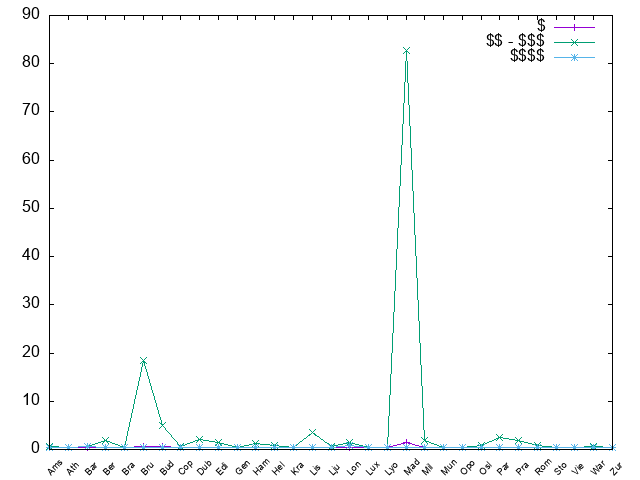
\includegraphics[width=0.8\textwidth]{images/graficoTempiRicorsione.png}
    \caption{Grafico tempi di ricorsione}
\end{figure}

\chapter{Valutazioni dei risultati ottenuti}\label{cap_valutazioni}

\section{Punti di forza}
Nel complesso, l'applicazione, grazie ad un interfaccia grafica intuitiva, risulta semplice da utilizzare ed è in grado di soddisfare le richieste dell'utente in tempi ragionevolmente brevi.

Un altro aspetto importante per il corretto funzionamento è la robustezza che caratterizza l'interazione con il data-set e con gli input dell'utente. Il programma, infatti, effettua un elevato numero di controlli sugli input ricevuti, evitando così di generare degli errori comportando l'arresto dell'esecuzione.

\section{Punti di debolezza}
Le criticità possono sorgere nel momento in cui l'utente selezioni particolari combinazioni di input che obbligano il programma ad aumentare esponenzialmente le operazioni da svolgere, rischiando di completare l'esecuzione in tempi elevati.

\section{Conclusioni}
Gli obiettivi del progetto sono, in conclusione, stati raggiunti: l'applicazione fornisce un utile strumento che semplifica la navigazione offrendo delle soluzioni personalizzate per ciascun utente.

\chapter{Licenza}

\includegraphics[width=4cm]{images/licenza.png}

Questo documento è condiviso con licenza Creative Commons BY-NC-SA 4.0.

Tu sei libero di:
\begin{itemize}
    \item Condividere — riprodurre, distribuire, comunicare al pubblico, esporre in pubblico, rappresentare, eseguire e recitare questo materiale con qualsiasi mezzo e formato
    \item Modificare — remixare, trasformare il materiale e basarti su di esso per le tue opere
\end{itemize}
Il licenziante non può revocare questi diritti fintanto che tu rispetti i termini della licenza.

Alle seguenti condizioni:
\begin{itemize}
    \item Attribuzione — Devi riconoscere una menzione di paternità adeguata , fornire un link alla licenza e indicare se sono state effettuate delle modifiche . Puoi fare ciò in qualsiasi maniera ragionevole possibile, ma non con modalità tali da suggerire che il licenziante avalli te o il tuo utilizzo del materiale.
    \item NonCommerciale — Non puoi utilizzare il materiale per scopi commerciali.
    \item StessaLicenza — Se remixi, trasformi il materiale o ti basi su di esso, devi distribuire i tuoi contributi con la stessa licenza del materiale originario.
    \item Divieto di restrizioni aggiuntive — Non puoi applicare termini legali o misure tecnologiche che impongano ad altri soggetti dei vincoli giuridici su quanto la licenza consente loro di fare.
\end{itemize}

Note:

Non sei tenuto a rispettare i termini della licenza per quelle componenti del materiale che siano in pubblico dominio o nei casi in cui il tuo utilizzo sia consentito da una eccezione o limitazione prevista dalla legge.

Non sono fornite garanzie. La licenza può non conferirti tutte le autorizzazioni necessarie per l'utilizzo che ti prefiggi. Ad esempio, diritti di terzi come i diritti all'immagine, alla riservatezza e i diritti morali potrebbero restringere gli usi che ti prefiggi sul materiale.

 Per una copia della licenza completa, visita \url{https://creativecommons.org/licenses/by-nc-sa/4.0/legalcode}
%%%%%%%%%%%%%%%%%%%%%%%%%%%%%%%%%%%%%%%%%%%%%%%%%%%%%%%%%%%
% Se serve la bibliografia
% \bibliographystyle{IEEEtran}
% \nocite{*}
% \bibliography{biblio}
%%%%%%%%%%%%%%%%%%%%%%%%%%%%%%%%%%%%%%%%%%%%%%%%%%%%%%%%%%%


\end{document}
